%-------------------------------------------
\begin{frame}[containsverbatim]
\frametitle{
\includegraphics[height=1cm]{shared/logo-github.png}}
%-------------------------------------------
\begin{block}{Sharing code with others}
Tools to share code (by sharing git repositories) with colleagues: GitHub, GitLab, and m... any others.\\
GitHub: so used that Microsoft was interested in it (\href{https://blogs.microsoft.com/blog/2018/06/04/microsoft-github-empowering-developers/}{\textcolor{blue}{\underline{bought}}} in june 2018)
Git-based: so all git concept and command are retained, \verb|git push| is the GitHub command for a "sharing step" \verb|git push|:
\begin{center}
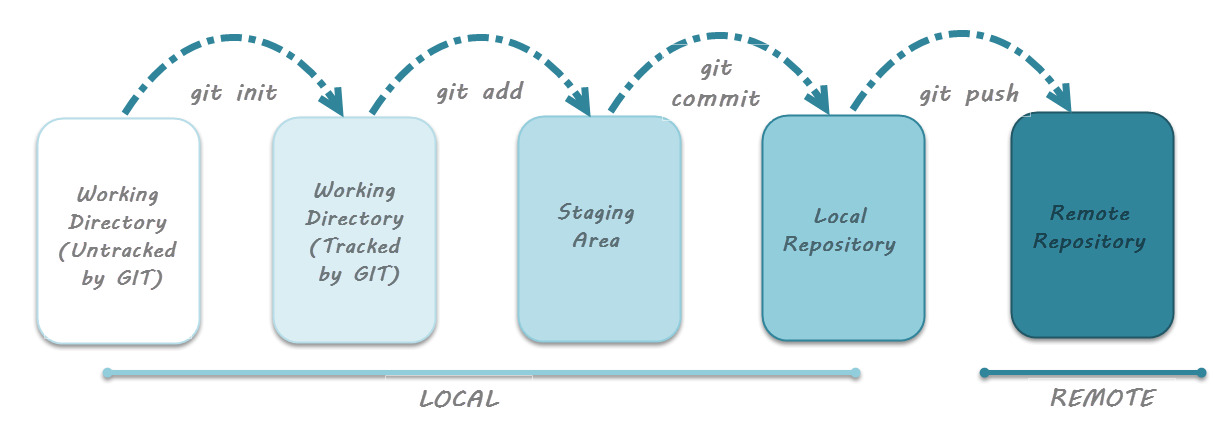
\includegraphics[height=3cm]{05_history/Images/FAIR_git-4push.png}
\end{center}
Web-based: graphical interface + many added functionalities
\end{block}
\end{frame}
%-------------------------------------------
\begin{frame}{
\includegraphics[height=1cm]{shared/logo-github.png} }
%-------------------------------------------
\begin{block}{Terminology}
\begin{itemize}
    \item user: your account on GitHub
    \item organization: account for one or more user (e.g., swcarpentry)
    \item local GitHub: copies of GitHub files located your computer
    \item remote GitHub: your GitHub files located on \href{https://github.com}{\textcolor{blue}{\underline{https://github.com}}}
    \item fork: a copy of a GitHub repository to your own GitHub account (git equivalent: clone)
    \item push: send changes on the working repository to your remote GitHub repository
    \item pull: copy changes on the remote GitHub repository to your local GitHub repository (useful when multiple people make changes)
    \item pull request: propose your changes to the initial forked GitHub repository. Like a place to compare and discuss the differences introduced on a branch with reviews, comments, integrated tests, etc
\end{itemize}
\end{block}
\end{frame}



%-------------------------------------------
\begin{frame}{GitHub development cycle}
%-------------------------------------------
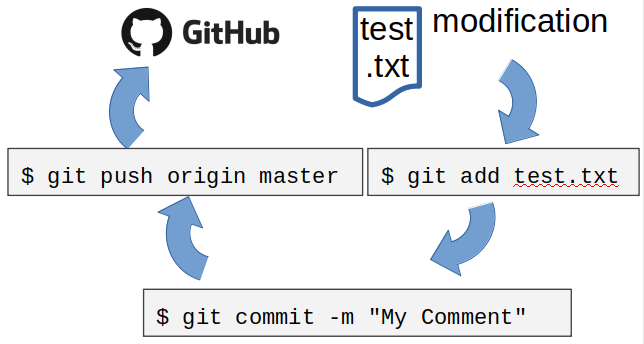
\includegraphics[height=5cm]{05_history/Images/FAIR_github_devCycle.png}
\end{frame}